\documentclass[12pt]{article}
\usepackage[letterpaper,top=0.9in,bottom=0.85in,left=0.75in,right=0.75in,
  headheight=16pt,headsep=0.25in,footskip=0.45in]{geometry}
\usepackage[T1]{fontenc}
\usepackage{tgheros}
\renewcommand{\familydefault}{\sfdefault}
\usepackage{tikz}
\usetikzlibrary{arrows.meta,calc}
\usepackage{fancyhdr}
\pagestyle{fancy}
\fancyhf{}
\fancyhead[L]{Week NN / Hidden armies / Grades 4--5}
\fancyfoot[L]{\small Bellingham Math Circle / Week NN / HA-45-v1}
\fancyfoot[R]{\small \thepage}
\renewcommand{\headrulewidth}{0.4pt}
\setlength{\parindent}{0pt}
\setlength{\parskip}{0pt}
\hyphenpenalty=10000
\exhyphenpenalty=10000
\newcommand{\prob}[1]{\par\vspace{16pt}\noindent\textbf{Problem #1:}\ }
\tikzset{sbox/.style={draw,line width=0.6pt,minimum width=#1,minimum height=0.5cm,
  inner sep=0pt,outer sep=0pt,font=\sffamily},sbox/.default=0.56cm}
% a plan strip written inline: cubes on hills 1, 2, 3
\newcommand{\strip}[4][0.56cm]{\hspace{1.5pt}\tikz[baseline={([yshift=-0.75ex]a.center)}]{%
  \node[sbox=#1] (a) {#2};\node[sbox=#1,anchor=west] (b) at (a.east) {#3};%
  \node[sbox=#1,anchor=west] (c) at (b.east) {#4};}\hspace{1.5pt}}
\begin{document}
\raggedright

\begin{minipage}[c]{0.55\linewidth}\raggedright Both players have the same number of cubes. Behind your folder, put all your cubes on the three hills of your mat. This is your plan. A hill can stay empty. Lift the folders at the same time. On each hill, the player with more cubes wins the hill and puts a token on it. If the cubes are equal, nobody wins that hill. The player who wins more hills wins the game. If both players win the same number of hills, the game is a tie. A plan is written as three numbers in a strip: the cubes on hills 1, 2 and 3.\end{minipage}\hfill\begin{minipage}[c]{0.42\linewidth}\centering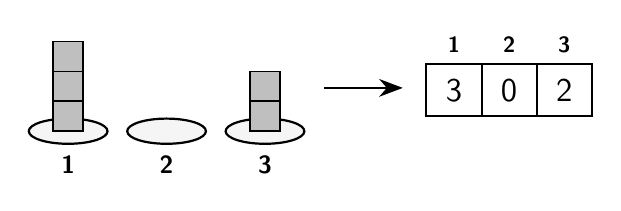
\begin{tikzpicture}[]
\draw[line width=0.8pt,fill=black!4] (0.000,0.000) ellipse (0.5 and 0.16);
\node[font=\small\bfseries] at (0.000,-0.430) {1};
\draw[line width=0.6pt,fill=black!25] (-0.190,0.000) rectangle (0.190,0.380);
\draw[line width=0.6pt,fill=black!25] (-0.190,0.380) rectangle (0.190,0.760);
\draw[line width=0.6pt,fill=black!25] (-0.190,0.760) rectangle (0.190,1.140);
\draw[line width=0.8pt,fill=black!4] (1.250,0.000) ellipse (0.5 and 0.16);
\node[font=\small\bfseries] at (1.250,-0.430) {2};
\draw[line width=0.8pt,fill=black!4] (2.500,0.000) ellipse (0.5 and 0.16);
\node[font=\small\bfseries] at (2.500,-0.430) {3};
\draw[line width=0.6pt,fill=black!25] (2.310,0.000) rectangle (2.690,0.380);
\draw[line width=0.6pt,fill=black!25] (2.310,0.380) rectangle (2.690,0.760);
\draw[-{Stealth[length=3mm]},line width=0.9pt] (3.25,0.55) -- (4.25,0.55);
\draw[line width=0.7pt] (4.550,0.190) rectangle (5.250,0.850);
\node[font=\large] at (4.900,0.520) {3};
\node[font=\footnotesize\bfseries] at (4.900,1.100) {1};
\draw[line width=0.7pt] (5.250,0.190) rectangle (5.950,0.850);
\node[font=\large] at (5.600,0.520) {0};
\node[font=\footnotesize\bfseries] at (5.600,1.100) {2};
\draw[line width=0.7pt] (5.950,0.190) rectangle (6.650,0.850);
\node[font=\large] at (6.300,0.520) {2};
\node[font=\footnotesize\bfseries] at (6.300,1.100) {3};
\end{tikzpicture}\end{minipage}

\prob{1}Play the game with 6 cubes each. Is there a plan that nobody can beat? To test a plan, one player shows it and the others try to beat it.
\par\vspace{12pt}\noindent\hspace*{0.3cm}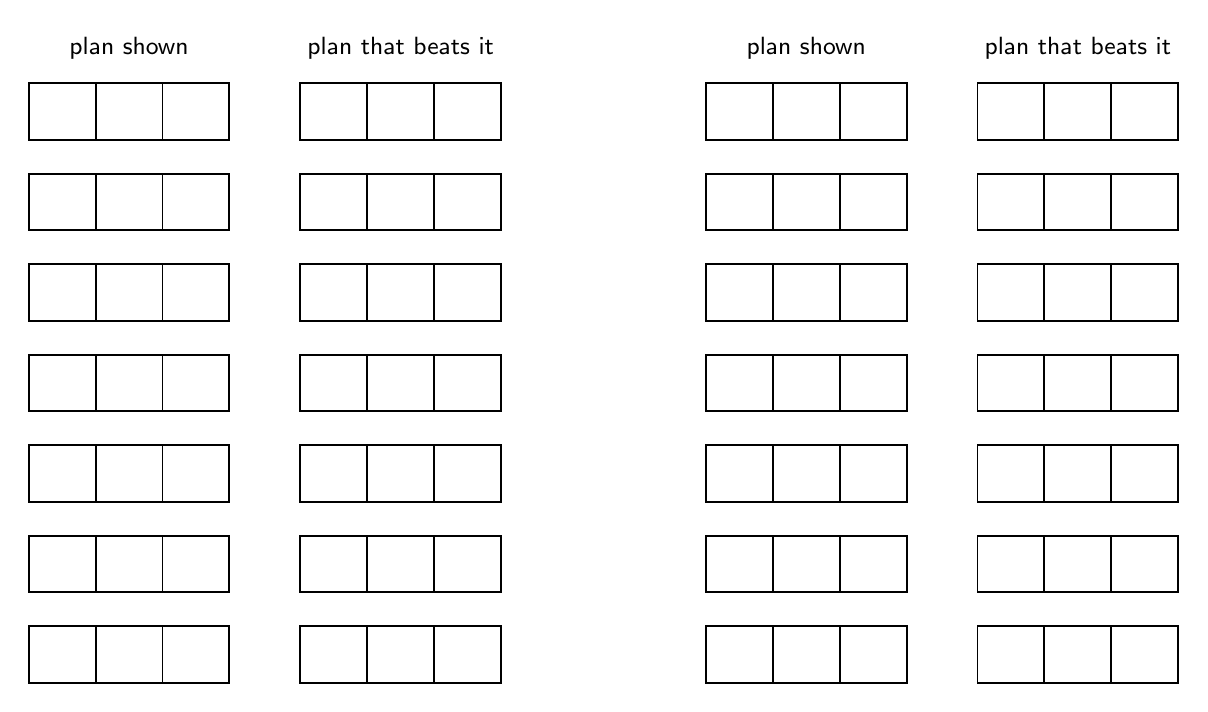
\begin{tikzpicture}[]
\node[font=\small,anchor=south] at (1.775,0.05) {plan shown};
\node[font=\small,anchor=south] at (5.225,0.05) {plan that beats it};
\draw[line width=0.7pt] (0.500,-0.850) rectangle (1.350,-0.130);
\draw[line width=0.7pt] (1.350,-0.850) rectangle (2.200,-0.130);
\draw[line width=0.7pt] (2.200,-0.850) rectangle (3.050,-0.130);
\draw[line width=0.7pt] (3.950,-0.850) rectangle (4.800,-0.130);
\draw[line width=0.7pt] (4.800,-0.850) rectangle (5.650,-0.130);
\draw[line width=0.7pt] (5.650,-0.850) rectangle (6.500,-0.130);
\draw[line width=0.7pt] (0.500,-2.000) rectangle (1.350,-1.280);
\draw[line width=0.7pt] (1.350,-2.000) rectangle (2.200,-1.280);
\draw[line width=0.7pt] (2.200,-2.000) rectangle (3.050,-1.280);
\draw[line width=0.7pt] (3.950,-2.000) rectangle (4.800,-1.280);
\draw[line width=0.7pt] (4.800,-2.000) rectangle (5.650,-1.280);
\draw[line width=0.7pt] (5.650,-2.000) rectangle (6.500,-1.280);
\draw[line width=0.7pt] (0.500,-3.150) rectangle (1.350,-2.430);
\draw[line width=0.7pt] (1.350,-3.150) rectangle (2.200,-2.430);
\draw[line width=0.7pt] (2.200,-3.150) rectangle (3.050,-2.430);
\draw[line width=0.7pt] (3.950,-3.150) rectangle (4.800,-2.430);
\draw[line width=0.7pt] (4.800,-3.150) rectangle (5.650,-2.430);
\draw[line width=0.7pt] (5.650,-3.150) rectangle (6.500,-2.430);
\draw[line width=0.7pt] (0.500,-4.300) rectangle (1.350,-3.580);
\draw[line width=0.7pt] (1.350,-4.300) rectangle (2.200,-3.580);
\draw[line width=0.7pt] (2.200,-4.300) rectangle (3.050,-3.580);
\draw[line width=0.7pt] (3.950,-4.300) rectangle (4.800,-3.580);
\draw[line width=0.7pt] (4.800,-4.300) rectangle (5.650,-3.580);
\draw[line width=0.7pt] (5.650,-4.300) rectangle (6.500,-3.580);
\draw[line width=0.7pt] (0.500,-5.450) rectangle (1.350,-4.730);
\draw[line width=0.7pt] (1.350,-5.450) rectangle (2.200,-4.730);
\draw[line width=0.7pt] (2.200,-5.450) rectangle (3.050,-4.730);
\draw[line width=0.7pt] (3.950,-5.450) rectangle (4.800,-4.730);
\draw[line width=0.7pt] (4.800,-5.450) rectangle (5.650,-4.730);
\draw[line width=0.7pt] (5.650,-5.450) rectangle (6.500,-4.730);
\draw[line width=0.7pt] (0.500,-6.600) rectangle (1.350,-5.880);
\draw[line width=0.7pt] (1.350,-6.600) rectangle (2.200,-5.880);
\draw[line width=0.7pt] (2.200,-6.600) rectangle (3.050,-5.880);
\draw[line width=0.7pt] (3.950,-6.600) rectangle (4.800,-5.880);
\draw[line width=0.7pt] (4.800,-6.600) rectangle (5.650,-5.880);
\draw[line width=0.7pt] (5.650,-6.600) rectangle (6.500,-5.880);
\draw[line width=0.7pt] (0.500,-7.750) rectangle (1.350,-7.030);
\draw[line width=0.7pt] (1.350,-7.750) rectangle (2.200,-7.030);
\draw[line width=0.7pt] (2.200,-7.750) rectangle (3.050,-7.030);
\draw[line width=0.7pt] (3.950,-7.750) rectangle (4.800,-7.030);
\draw[line width=0.7pt] (4.800,-7.750) rectangle (5.650,-7.030);
\draw[line width=0.7pt] (5.650,-7.750) rectangle (6.500,-7.030);
\node[font=\small,anchor=south] at (10.375,0.05) {plan shown};
\node[font=\small,anchor=south] at (13.825,0.05) {plan that beats it};
\draw[line width=0.7pt] (9.100,-0.850) rectangle (9.950,-0.130);
\draw[line width=0.7pt] (9.950,-0.850) rectangle (10.800,-0.130);
\draw[line width=0.7pt] (10.800,-0.850) rectangle (11.650,-0.130);
\draw[line width=0.7pt] (12.550,-0.850) rectangle (13.400,-0.130);
\draw[line width=0.7pt] (13.400,-0.850) rectangle (14.250,-0.130);
\draw[line width=0.7pt] (14.250,-0.850) rectangle (15.100,-0.130);
\draw[line width=0.7pt] (9.100,-2.000) rectangle (9.950,-1.280);
\draw[line width=0.7pt] (9.950,-2.000) rectangle (10.800,-1.280);
\draw[line width=0.7pt] (10.800,-2.000) rectangle (11.650,-1.280);
\draw[line width=0.7pt] (12.550,-2.000) rectangle (13.400,-1.280);
\draw[line width=0.7pt] (13.400,-2.000) rectangle (14.250,-1.280);
\draw[line width=0.7pt] (14.250,-2.000) rectangle (15.100,-1.280);
\draw[line width=0.7pt] (9.100,-3.150) rectangle (9.950,-2.430);
\draw[line width=0.7pt] (9.950,-3.150) rectangle (10.800,-2.430);
\draw[line width=0.7pt] (10.800,-3.150) rectangle (11.650,-2.430);
\draw[line width=0.7pt] (12.550,-3.150) rectangle (13.400,-2.430);
\draw[line width=0.7pt] (13.400,-3.150) rectangle (14.250,-2.430);
\draw[line width=0.7pt] (14.250,-3.150) rectangle (15.100,-2.430);
\draw[line width=0.7pt] (9.100,-4.300) rectangle (9.950,-3.580);
\draw[line width=0.7pt] (9.950,-4.300) rectangle (10.800,-3.580);
\draw[line width=0.7pt] (10.800,-4.300) rectangle (11.650,-3.580);
\draw[line width=0.7pt] (12.550,-4.300) rectangle (13.400,-3.580);
\draw[line width=0.7pt] (13.400,-4.300) rectangle (14.250,-3.580);
\draw[line width=0.7pt] (14.250,-4.300) rectangle (15.100,-3.580);
\draw[line width=0.7pt] (9.100,-5.450) rectangle (9.950,-4.730);
\draw[line width=0.7pt] (9.950,-5.450) rectangle (10.800,-4.730);
\draw[line width=0.7pt] (10.800,-5.450) rectangle (11.650,-4.730);
\draw[line width=0.7pt] (12.550,-5.450) rectangle (13.400,-4.730);
\draw[line width=0.7pt] (13.400,-5.450) rectangle (14.250,-4.730);
\draw[line width=0.7pt] (14.250,-5.450) rectangle (15.100,-4.730);
\draw[line width=0.7pt] (9.100,-6.600) rectangle (9.950,-5.880);
\draw[line width=0.7pt] (9.950,-6.600) rectangle (10.800,-5.880);
\draw[line width=0.7pt] (10.800,-6.600) rectangle (11.650,-5.880);
\draw[line width=0.7pt] (12.550,-6.600) rectangle (13.400,-5.880);
\draw[line width=0.7pt] (13.400,-6.600) rectangle (14.250,-5.880);
\draw[line width=0.7pt] (14.250,-6.600) rectangle (15.100,-5.880);
\draw[line width=0.7pt] (9.100,-7.750) rectangle (9.950,-7.030);
\draw[line width=0.7pt] (9.950,-7.750) rectangle (10.800,-7.030);
\draw[line width=0.7pt] (10.800,-7.750) rectangle (11.650,-7.030);
\draw[line width=0.7pt] (12.550,-7.750) rectangle (13.400,-7.030);
\draw[line width=0.7pt] (13.400,-7.750) rectangle (14.250,-7.030);
\draw[line width=0.7pt] (14.250,-7.750) rectangle (15.100,-7.030);
\end{tikzpicture}
\newpage
\prob{2}Beat each plan below. Then explain a way to beat any plan with 6 or more cubes that your partner names.
\par\vspace{12pt}\noindent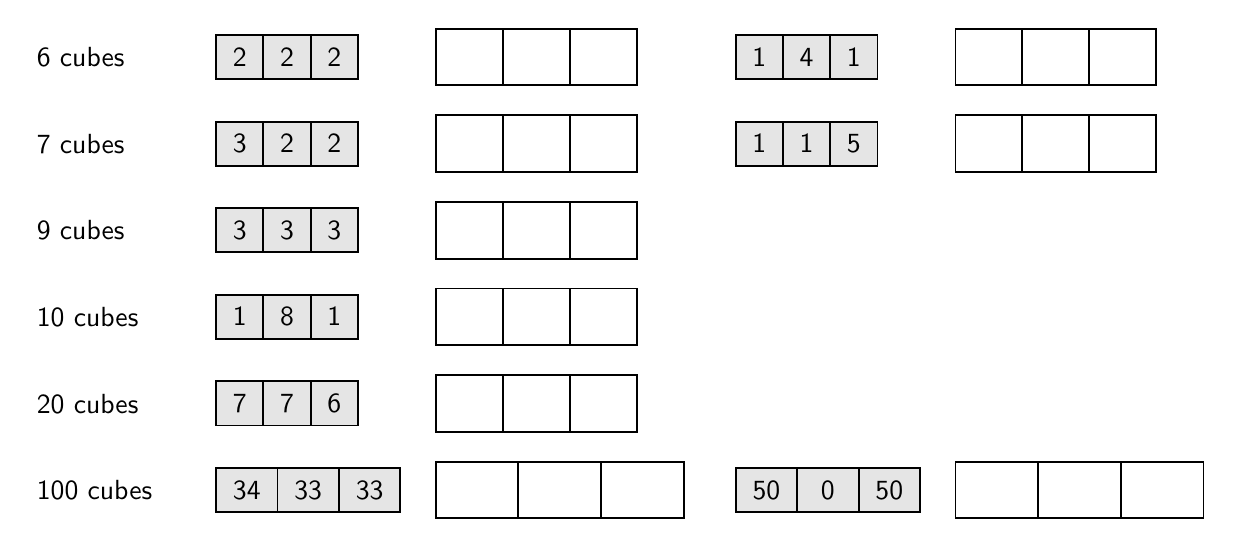
\begin{tikzpicture}[]
\node[anchor=west,font=\normalsize] at (0,0.360) {6 cubes};
\draw[line width=0.7pt,fill=black!10] (2.400,0.080) rectangle (3.000,0.640);
\node[font=\normalsize] at (2.700,0.360) {2};
\draw[line width=0.7pt,fill=black!10] (3.000,0.080) rectangle (3.600,0.640);
\node[font=\normalsize] at (3.300,0.360) {2};
\draw[line width=0.7pt,fill=black!10] (3.600,0.080) rectangle (4.200,0.640);
\node[font=\normalsize] at (3.900,0.360) {2};
\draw[line width=0.7pt] (5.190,0.000) rectangle (6.040,0.720);
\draw[line width=0.7pt] (6.040,0.000) rectangle (6.890,0.720);
\draw[line width=0.7pt] (6.890,0.000) rectangle (7.740,0.720);
\draw[line width=0.7pt,fill=black!10] (9.000,0.080) rectangle (9.600,0.640);
\node[font=\normalsize] at (9.300,0.360) {1};
\draw[line width=0.7pt,fill=black!10] (9.600,0.080) rectangle (10.200,0.640);
\node[font=\normalsize] at (9.900,0.360) {4};
\draw[line width=0.7pt,fill=black!10] (10.200,0.080) rectangle (10.800,0.640);
\node[font=\normalsize] at (10.500,0.360) {1};
\draw[line width=0.7pt] (11.790,0.000) rectangle (12.640,0.720);
\draw[line width=0.7pt] (12.640,0.000) rectangle (13.490,0.720);
\draw[line width=0.7pt] (13.490,0.000) rectangle (14.340,0.720);
\node[anchor=west,font=\normalsize] at (0,-0.740) {7 cubes};
\draw[line width=0.7pt,fill=black!10] (2.400,-1.020) rectangle (3.000,-0.460);
\node[font=\normalsize] at (2.700,-0.740) {3};
\draw[line width=0.7pt,fill=black!10] (3.000,-1.020) rectangle (3.600,-0.460);
\node[font=\normalsize] at (3.300,-0.740) {2};
\draw[line width=0.7pt,fill=black!10] (3.600,-1.020) rectangle (4.200,-0.460);
\node[font=\normalsize] at (3.900,-0.740) {2};
\draw[line width=0.7pt] (5.190,-1.100) rectangle (6.040,-0.380);
\draw[line width=0.7pt] (6.040,-1.100) rectangle (6.890,-0.380);
\draw[line width=0.7pt] (6.890,-1.100) rectangle (7.740,-0.380);
\draw[line width=0.7pt,fill=black!10] (9.000,-1.020) rectangle (9.600,-0.460);
\node[font=\normalsize] at (9.300,-0.740) {1};
\draw[line width=0.7pt,fill=black!10] (9.600,-1.020) rectangle (10.200,-0.460);
\node[font=\normalsize] at (9.900,-0.740) {1};
\draw[line width=0.7pt,fill=black!10] (10.200,-1.020) rectangle (10.800,-0.460);
\node[font=\normalsize] at (10.500,-0.740) {5};
\draw[line width=0.7pt] (11.790,-1.100) rectangle (12.640,-0.380);
\draw[line width=0.7pt] (12.640,-1.100) rectangle (13.490,-0.380);
\draw[line width=0.7pt] (13.490,-1.100) rectangle (14.340,-0.380);
\node[anchor=west,font=\normalsize] at (0,-1.840) {9 cubes};
\draw[line width=0.7pt,fill=black!10] (2.400,-2.120) rectangle (3.000,-1.560);
\node[font=\normalsize] at (2.700,-1.840) {3};
\draw[line width=0.7pt,fill=black!10] (3.000,-2.120) rectangle (3.600,-1.560);
\node[font=\normalsize] at (3.300,-1.840) {3};
\draw[line width=0.7pt,fill=black!10] (3.600,-2.120) rectangle (4.200,-1.560);
\node[font=\normalsize] at (3.900,-1.840) {3};
\draw[line width=0.7pt] (5.190,-2.200) rectangle (6.040,-1.480);
\draw[line width=0.7pt] (6.040,-2.200) rectangle (6.890,-1.480);
\draw[line width=0.7pt] (6.890,-2.200) rectangle (7.740,-1.480);
\node[anchor=west,font=\normalsize] at (0,-2.940) {10 cubes};
\draw[line width=0.7pt,fill=black!10] (2.400,-3.220) rectangle (3.000,-2.660);
\node[font=\normalsize] at (2.700,-2.940) {1};
\draw[line width=0.7pt,fill=black!10] (3.000,-3.220) rectangle (3.600,-2.660);
\node[font=\normalsize] at (3.300,-2.940) {8};
\draw[line width=0.7pt,fill=black!10] (3.600,-3.220) rectangle (4.200,-2.660);
\node[font=\normalsize] at (3.900,-2.940) {1};
\draw[line width=0.7pt] (5.190,-3.300) rectangle (6.040,-2.580);
\draw[line width=0.7pt] (6.040,-3.300) rectangle (6.890,-2.580);
\draw[line width=0.7pt] (6.890,-3.300) rectangle (7.740,-2.580);
\node[anchor=west,font=\normalsize] at (0,-4.040) {20 cubes};
\draw[line width=0.7pt,fill=black!10] (2.400,-4.320) rectangle (3.000,-3.760);
\node[font=\normalsize] at (2.700,-4.040) {7};
\draw[line width=0.7pt,fill=black!10] (3.000,-4.320) rectangle (3.600,-3.760);
\node[font=\normalsize] at (3.300,-4.040) {7};
\draw[line width=0.7pt,fill=black!10] (3.600,-4.320) rectangle (4.200,-3.760);
\node[font=\normalsize] at (3.900,-4.040) {6};
\draw[line width=0.7pt] (5.190,-4.400) rectangle (6.040,-3.680);
\draw[line width=0.7pt] (6.040,-4.400) rectangle (6.890,-3.680);
\draw[line width=0.7pt] (6.890,-4.400) rectangle (7.740,-3.680);
\node[anchor=west,font=\normalsize] at (0,-5.140) {100 cubes};
\draw[line width=0.7pt,fill=black!10] (2.400,-5.420) rectangle (3.180,-4.860);
\node[font=\normalsize] at (2.790,-5.140) {34};
\draw[line width=0.7pt,fill=black!10] (3.180,-5.420) rectangle (3.960,-4.860);
\node[font=\normalsize] at (3.570,-5.140) {33};
\draw[line width=0.7pt,fill=black!10] (3.960,-5.420) rectangle (4.740,-4.860);
\node[font=\normalsize] at (4.350,-5.140) {33};
\draw[line width=0.7pt] (5.190,-5.500) rectangle (6.240,-4.780);
\draw[line width=0.7pt] (6.240,-5.500) rectangle (7.290,-4.780);
\draw[line width=0.7pt] (7.290,-5.500) rectangle (8.340,-4.780);
\draw[line width=0.7pt,fill=black!10] (9.000,-5.420) rectangle (9.780,-4.860);
\node[font=\normalsize] at (9.390,-5.140) {50};
\draw[line width=0.7pt,fill=black!10] (9.780,-5.420) rectangle (10.560,-4.860);
\node[font=\normalsize] at (10.170,-5.140) {0};
\draw[line width=0.7pt,fill=black!10] (10.560,-5.420) rectangle (11.340,-4.860);
\node[font=\normalsize] at (10.950,-5.140) {50};
\draw[line width=0.7pt] (11.790,-5.500) rectangle (12.840,-4.780);
\draw[line width=0.7pt] (12.840,-5.500) rectangle (13.890,-4.780);
\draw[line width=0.7pt] (13.890,-5.500) rectangle (14.940,-4.780);
\end{tikzpicture}
\par\vspace{10pt}\par\noindent
\begin{tikzpicture}\draw[black!30,line width=0.5pt] (0,-0.850) -- (\linewidth-1pt,-0.850);\draw[black!30,line width=0.5pt] (0,-1.700) -- (\linewidth-1pt,-1.700);\draw[black!30,line width=0.5pt] (0,-2.550) -- (\linewidth-1pt,-2.550);\draw[black!30,line width=0.5pt] (0,-3.400) -- (\linewidth-1pt,-3.400);\draw[black!30,line width=0.5pt] (0,-4.250) -- (\linewidth-1pt,-4.250);\draw[black!30,line width=0.5pt] (0,-5.100) -- (\linewidth-1pt,-5.100);\end{tikzpicture}\par
\prob{3}For which numbers of cubes is there a plan that nobody can beat? Explain.
\par\vspace{2pt}\par\noindent
\begin{tikzpicture}\draw[black!30,line width=0.5pt] (0,-0.850) -- (\linewidth-1pt,-0.850);\draw[black!30,line width=0.5pt] (0,-1.700) -- (\linewidth-1pt,-1.700);\draw[black!30,line width=0.5pt] (0,-2.550) -- (\linewidth-1pt,-2.550);\draw[black!30,line width=0.5pt] (0,-3.400) -- (\linewidth-1pt,-3.400);\draw[black!30,line width=0.5pt] (0,-4.250) -- (\linewidth-1pt,-4.250);\draw[black!30,line width=0.5pt] (0,-5.100) -- (\linewidth-1pt,-5.100);\draw[black!30,line width=0.5pt] (0,-5.950) -- (\linewidth-1pt,-5.950);\draw[black!30,line width=0.5pt] (0,-6.800) -- (\linewidth-1pt,-6.800);\end{tikzpicture}\par
\newpage
\prob{4}There are 28 plans with 6 cubes. For each one, find how many of the 28 plans it beats. Share the work. Which plans beat the most? Which beat the fewest?
\par\vspace{16pt}\noindent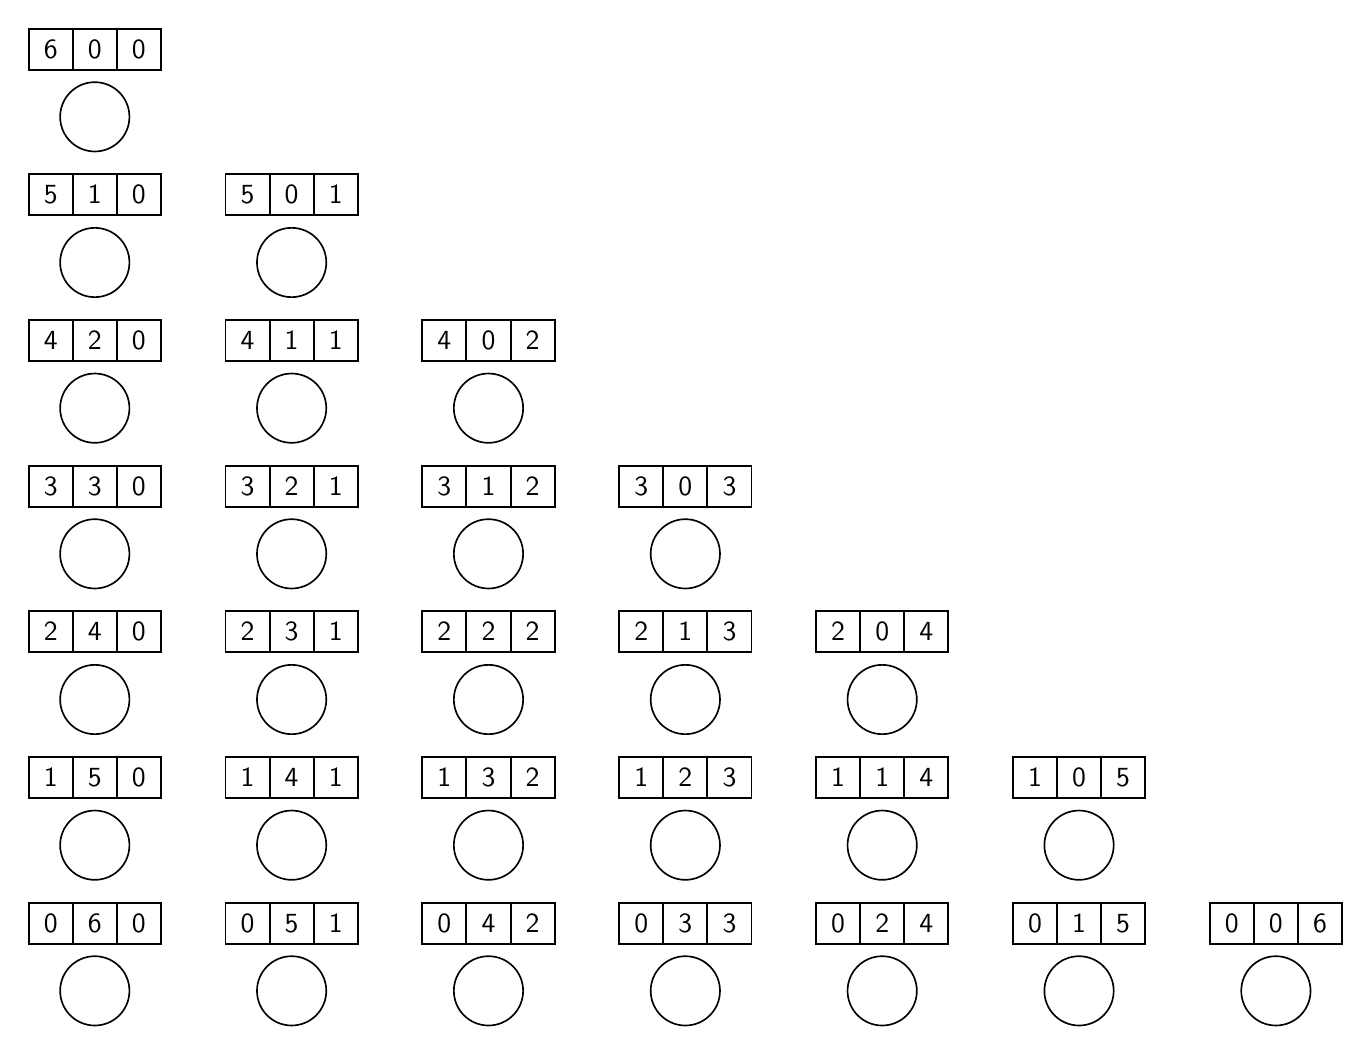
\begin{tikzpicture}[]
\draw[line width=0.7pt] (0.100,0.000) rectangle (0.660,0.520);
\node[font=\normalsize] at (0.380,0.260) {6};
\draw[line width=0.7pt] (0.660,0.000) rectangle (1.220,0.520);
\node[font=\normalsize] at (0.940,0.260) {0};
\draw[line width=0.7pt] (1.220,0.000) rectangle (1.780,0.520);
\node[font=\normalsize] at (1.500,0.260) {0};
\draw[line width=0.6pt] (0.940,-0.600) circle (0.44);
\draw[line width=0.7pt] (0.100,-1.850) rectangle (0.660,-1.330);
\node[font=\normalsize] at (0.380,-1.590) {5};
\draw[line width=0.7pt] (0.660,-1.850) rectangle (1.220,-1.330);
\node[font=\normalsize] at (0.940,-1.590) {1};
\draw[line width=0.7pt] (1.220,-1.850) rectangle (1.780,-1.330);
\node[font=\normalsize] at (1.500,-1.590) {0};
\draw[line width=0.6pt] (0.940,-2.450) circle (0.44);
\draw[line width=0.7pt] (2.600,-1.850) rectangle (3.160,-1.330);
\node[font=\normalsize] at (2.880,-1.590) {5};
\draw[line width=0.7pt] (3.160,-1.850) rectangle (3.720,-1.330);
\node[font=\normalsize] at (3.440,-1.590) {0};
\draw[line width=0.7pt] (3.720,-1.850) rectangle (4.280,-1.330);
\node[font=\normalsize] at (4.000,-1.590) {1};
\draw[line width=0.6pt] (3.440,-2.450) circle (0.44);
\draw[line width=0.7pt] (0.100,-3.700) rectangle (0.660,-3.180);
\node[font=\normalsize] at (0.380,-3.440) {4};
\draw[line width=0.7pt] (0.660,-3.700) rectangle (1.220,-3.180);
\node[font=\normalsize] at (0.940,-3.440) {2};
\draw[line width=0.7pt] (1.220,-3.700) rectangle (1.780,-3.180);
\node[font=\normalsize] at (1.500,-3.440) {0};
\draw[line width=0.6pt] (0.940,-4.300) circle (0.44);
\draw[line width=0.7pt] (2.600,-3.700) rectangle (3.160,-3.180);
\node[font=\normalsize] at (2.880,-3.440) {4};
\draw[line width=0.7pt] (3.160,-3.700) rectangle (3.720,-3.180);
\node[font=\normalsize] at (3.440,-3.440) {1};
\draw[line width=0.7pt] (3.720,-3.700) rectangle (4.280,-3.180);
\node[font=\normalsize] at (4.000,-3.440) {1};
\draw[line width=0.6pt] (3.440,-4.300) circle (0.44);
\draw[line width=0.7pt] (5.100,-3.700) rectangle (5.660,-3.180);
\node[font=\normalsize] at (5.380,-3.440) {4};
\draw[line width=0.7pt] (5.660,-3.700) rectangle (6.220,-3.180);
\node[font=\normalsize] at (5.940,-3.440) {0};
\draw[line width=0.7pt] (6.220,-3.700) rectangle (6.780,-3.180);
\node[font=\normalsize] at (6.500,-3.440) {2};
\draw[line width=0.6pt] (5.940,-4.300) circle (0.44);
\draw[line width=0.7pt] (0.100,-5.550) rectangle (0.660,-5.030);
\node[font=\normalsize] at (0.380,-5.290) {3};
\draw[line width=0.7pt] (0.660,-5.550) rectangle (1.220,-5.030);
\node[font=\normalsize] at (0.940,-5.290) {3};
\draw[line width=0.7pt] (1.220,-5.550) rectangle (1.780,-5.030);
\node[font=\normalsize] at (1.500,-5.290) {0};
\draw[line width=0.6pt] (0.940,-6.150) circle (0.44);
\draw[line width=0.7pt] (2.600,-5.550) rectangle (3.160,-5.030);
\node[font=\normalsize] at (2.880,-5.290) {3};
\draw[line width=0.7pt] (3.160,-5.550) rectangle (3.720,-5.030);
\node[font=\normalsize] at (3.440,-5.290) {2};
\draw[line width=0.7pt] (3.720,-5.550) rectangle (4.280,-5.030);
\node[font=\normalsize] at (4.000,-5.290) {1};
\draw[line width=0.6pt] (3.440,-6.150) circle (0.44);
\draw[line width=0.7pt] (5.100,-5.550) rectangle (5.660,-5.030);
\node[font=\normalsize] at (5.380,-5.290) {3};
\draw[line width=0.7pt] (5.660,-5.550) rectangle (6.220,-5.030);
\node[font=\normalsize] at (5.940,-5.290) {1};
\draw[line width=0.7pt] (6.220,-5.550) rectangle (6.780,-5.030);
\node[font=\normalsize] at (6.500,-5.290) {2};
\draw[line width=0.6pt] (5.940,-6.150) circle (0.44);
\draw[line width=0.7pt] (7.600,-5.550) rectangle (8.160,-5.030);
\node[font=\normalsize] at (7.880,-5.290) {3};
\draw[line width=0.7pt] (8.160,-5.550) rectangle (8.720,-5.030);
\node[font=\normalsize] at (8.440,-5.290) {0};
\draw[line width=0.7pt] (8.720,-5.550) rectangle (9.280,-5.030);
\node[font=\normalsize] at (9.000,-5.290) {3};
\draw[line width=0.6pt] (8.440,-6.150) circle (0.44);
\draw[line width=0.7pt] (0.100,-7.400) rectangle (0.660,-6.880);
\node[font=\normalsize] at (0.380,-7.140) {2};
\draw[line width=0.7pt] (0.660,-7.400) rectangle (1.220,-6.880);
\node[font=\normalsize] at (0.940,-7.140) {4};
\draw[line width=0.7pt] (1.220,-7.400) rectangle (1.780,-6.880);
\node[font=\normalsize] at (1.500,-7.140) {0};
\draw[line width=0.6pt] (0.940,-8.000) circle (0.44);
\draw[line width=0.7pt] (2.600,-7.400) rectangle (3.160,-6.880);
\node[font=\normalsize] at (2.880,-7.140) {2};
\draw[line width=0.7pt] (3.160,-7.400) rectangle (3.720,-6.880);
\node[font=\normalsize] at (3.440,-7.140) {3};
\draw[line width=0.7pt] (3.720,-7.400) rectangle (4.280,-6.880);
\node[font=\normalsize] at (4.000,-7.140) {1};
\draw[line width=0.6pt] (3.440,-8.000) circle (0.44);
\draw[line width=0.7pt] (5.100,-7.400) rectangle (5.660,-6.880);
\node[font=\normalsize] at (5.380,-7.140) {2};
\draw[line width=0.7pt] (5.660,-7.400) rectangle (6.220,-6.880);
\node[font=\normalsize] at (5.940,-7.140) {2};
\draw[line width=0.7pt] (6.220,-7.400) rectangle (6.780,-6.880);
\node[font=\normalsize] at (6.500,-7.140) {2};
\draw[line width=0.6pt] (5.940,-8.000) circle (0.44);
\draw[line width=0.7pt] (7.600,-7.400) rectangle (8.160,-6.880);
\node[font=\normalsize] at (7.880,-7.140) {2};
\draw[line width=0.7pt] (8.160,-7.400) rectangle (8.720,-6.880);
\node[font=\normalsize] at (8.440,-7.140) {1};
\draw[line width=0.7pt] (8.720,-7.400) rectangle (9.280,-6.880);
\node[font=\normalsize] at (9.000,-7.140) {3};
\draw[line width=0.6pt] (8.440,-8.000) circle (0.44);
\draw[line width=0.7pt] (10.100,-7.400) rectangle (10.660,-6.880);
\node[font=\normalsize] at (10.380,-7.140) {2};
\draw[line width=0.7pt] (10.660,-7.400) rectangle (11.220,-6.880);
\node[font=\normalsize] at (10.940,-7.140) {0};
\draw[line width=0.7pt] (11.220,-7.400) rectangle (11.780,-6.880);
\node[font=\normalsize] at (11.500,-7.140) {4};
\draw[line width=0.6pt] (10.940,-8.000) circle (0.44);
\draw[line width=0.7pt] (0.100,-9.250) rectangle (0.660,-8.730);
\node[font=\normalsize] at (0.380,-8.990) {1};
\draw[line width=0.7pt] (0.660,-9.250) rectangle (1.220,-8.730);
\node[font=\normalsize] at (0.940,-8.990) {5};
\draw[line width=0.7pt] (1.220,-9.250) rectangle (1.780,-8.730);
\node[font=\normalsize] at (1.500,-8.990) {0};
\draw[line width=0.6pt] (0.940,-9.850) circle (0.44);
\draw[line width=0.7pt] (2.600,-9.250) rectangle (3.160,-8.730);
\node[font=\normalsize] at (2.880,-8.990) {1};
\draw[line width=0.7pt] (3.160,-9.250) rectangle (3.720,-8.730);
\node[font=\normalsize] at (3.440,-8.990) {4};
\draw[line width=0.7pt] (3.720,-9.250) rectangle (4.280,-8.730);
\node[font=\normalsize] at (4.000,-8.990) {1};
\draw[line width=0.6pt] (3.440,-9.850) circle (0.44);
\draw[line width=0.7pt] (5.100,-9.250) rectangle (5.660,-8.730);
\node[font=\normalsize] at (5.380,-8.990) {1};
\draw[line width=0.7pt] (5.660,-9.250) rectangle (6.220,-8.730);
\node[font=\normalsize] at (5.940,-8.990) {3};
\draw[line width=0.7pt] (6.220,-9.250) rectangle (6.780,-8.730);
\node[font=\normalsize] at (6.500,-8.990) {2};
\draw[line width=0.6pt] (5.940,-9.850) circle (0.44);
\draw[line width=0.7pt] (7.600,-9.250) rectangle (8.160,-8.730);
\node[font=\normalsize] at (7.880,-8.990) {1};
\draw[line width=0.7pt] (8.160,-9.250) rectangle (8.720,-8.730);
\node[font=\normalsize] at (8.440,-8.990) {2};
\draw[line width=0.7pt] (8.720,-9.250) rectangle (9.280,-8.730);
\node[font=\normalsize] at (9.000,-8.990) {3};
\draw[line width=0.6pt] (8.440,-9.850) circle (0.44);
\draw[line width=0.7pt] (10.100,-9.250) rectangle (10.660,-8.730);
\node[font=\normalsize] at (10.380,-8.990) {1};
\draw[line width=0.7pt] (10.660,-9.250) rectangle (11.220,-8.730);
\node[font=\normalsize] at (10.940,-8.990) {1};
\draw[line width=0.7pt] (11.220,-9.250) rectangle (11.780,-8.730);
\node[font=\normalsize] at (11.500,-8.990) {4};
\draw[line width=0.6pt] (10.940,-9.850) circle (0.44);
\draw[line width=0.7pt] (12.600,-9.250) rectangle (13.160,-8.730);
\node[font=\normalsize] at (12.880,-8.990) {1};
\draw[line width=0.7pt] (13.160,-9.250) rectangle (13.720,-8.730);
\node[font=\normalsize] at (13.440,-8.990) {0};
\draw[line width=0.7pt] (13.720,-9.250) rectangle (14.280,-8.730);
\node[font=\normalsize] at (14.000,-8.990) {5};
\draw[line width=0.6pt] (13.440,-9.850) circle (0.44);
\draw[line width=0.7pt] (0.100,-11.100) rectangle (0.660,-10.580);
\node[font=\normalsize] at (0.380,-10.840) {0};
\draw[line width=0.7pt] (0.660,-11.100) rectangle (1.220,-10.580);
\node[font=\normalsize] at (0.940,-10.840) {6};
\draw[line width=0.7pt] (1.220,-11.100) rectangle (1.780,-10.580);
\node[font=\normalsize] at (1.500,-10.840) {0};
\draw[line width=0.6pt] (0.940,-11.700) circle (0.44);
\draw[line width=0.7pt] (2.600,-11.100) rectangle (3.160,-10.580);
\node[font=\normalsize] at (2.880,-10.840) {0};
\draw[line width=0.7pt] (3.160,-11.100) rectangle (3.720,-10.580);
\node[font=\normalsize] at (3.440,-10.840) {5};
\draw[line width=0.7pt] (3.720,-11.100) rectangle (4.280,-10.580);
\node[font=\normalsize] at (4.000,-10.840) {1};
\draw[line width=0.6pt] (3.440,-11.700) circle (0.44);
\draw[line width=0.7pt] (5.100,-11.100) rectangle (5.660,-10.580);
\node[font=\normalsize] at (5.380,-10.840) {0};
\draw[line width=0.7pt] (5.660,-11.100) rectangle (6.220,-10.580);
\node[font=\normalsize] at (5.940,-10.840) {4};
\draw[line width=0.7pt] (6.220,-11.100) rectangle (6.780,-10.580);
\node[font=\normalsize] at (6.500,-10.840) {2};
\draw[line width=0.6pt] (5.940,-11.700) circle (0.44);
\draw[line width=0.7pt] (7.600,-11.100) rectangle (8.160,-10.580);
\node[font=\normalsize] at (7.880,-10.840) {0};
\draw[line width=0.7pt] (8.160,-11.100) rectangle (8.720,-10.580);
\node[font=\normalsize] at (8.440,-10.840) {3};
\draw[line width=0.7pt] (8.720,-11.100) rectangle (9.280,-10.580);
\node[font=\normalsize] at (9.000,-10.840) {3};
\draw[line width=0.6pt] (8.440,-11.700) circle (0.44);
\draw[line width=0.7pt] (10.100,-11.100) rectangle (10.660,-10.580);
\node[font=\normalsize] at (10.380,-10.840) {0};
\draw[line width=0.7pt] (10.660,-11.100) rectangle (11.220,-10.580);
\node[font=\normalsize] at (10.940,-10.840) {2};
\draw[line width=0.7pt] (11.220,-11.100) rectangle (11.780,-10.580);
\node[font=\normalsize] at (11.500,-10.840) {4};
\draw[line width=0.6pt] (10.940,-11.700) circle (0.44);
\draw[line width=0.7pt] (12.600,-11.100) rectangle (13.160,-10.580);
\node[font=\normalsize] at (12.880,-10.840) {0};
\draw[line width=0.7pt] (13.160,-11.100) rectangle (13.720,-10.580);
\node[font=\normalsize] at (13.440,-10.840) {1};
\draw[line width=0.7pt] (13.720,-11.100) rectangle (14.280,-10.580);
\node[font=\normalsize] at (14.000,-10.840) {5};
\draw[line width=0.6pt] (13.440,-11.700) circle (0.44);
\draw[line width=0.7pt] (15.100,-11.100) rectangle (15.660,-10.580);
\node[font=\normalsize] at (15.380,-10.840) {0};
\draw[line width=0.7pt] (15.660,-11.100) rectangle (16.220,-10.580);
\node[font=\normalsize] at (15.940,-10.840) {0};
\draw[line width=0.7pt] (16.220,-11.100) rectangle (16.780,-10.580);
\node[font=\normalsize] at (16.500,-10.840) {6};
\draw[line width=0.6pt] (15.940,-11.700) circle (0.44);
\end{tikzpicture}
\par\vspace{12pt}\par\noindent
\begin{tikzpicture}\draw[black!30,line width=0.5pt] (0,-0.850) -- (\linewidth-1pt,-0.850);\draw[black!30,line width=0.5pt] (0,-1.700) -- (\linewidth-1pt,-1.700);\draw[black!30,line width=0.5pt] (0,-2.550) -- (\linewidth-1pt,-2.550);\draw[black!30,line width=0.5pt] (0,-3.400) -- (\linewidth-1pt,-3.400);\draw[black!30,line width=0.5pt] (0,-4.250) -- (\linewidth-1pt,-4.250);\end{tikzpicture}\par
\newpage
\prob{5}Find three plans with 6 cubes so that each plan beats the next one around the circle. Which plans with 6 cubes can be part of a circle like this, and which cannot? Explain why.
\par\vspace{16pt}\noindent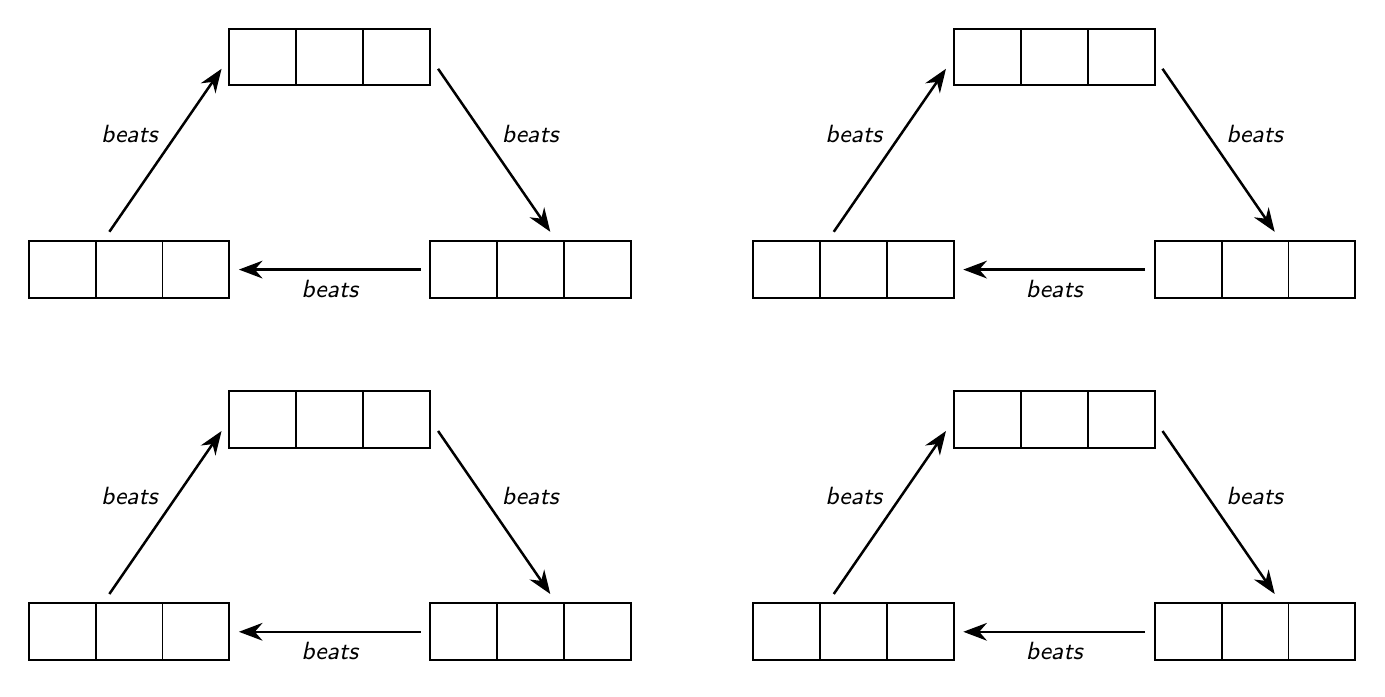
\begin{tikzpicture}[]
\draw[line width=0.7pt] (2.825,0.990) rectangle (3.675,1.710);
\draw[line width=0.7pt] (3.675,0.990) rectangle (4.525,1.710);
\draw[line width=0.7pt] (4.525,0.990) rectangle (5.375,1.710);
\draw[line width=0.7pt] (5.375,-1.710) rectangle (6.225,-0.990);
\draw[line width=0.7pt] (6.225,-1.710) rectangle (7.075,-0.990);
\draw[line width=0.7pt] (7.075,-1.710) rectangle (7.925,-0.990);
\draw[line width=0.7pt] (0.275,-1.710) rectangle (1.125,-0.990);
\draw[line width=0.7pt] (1.125,-1.710) rectangle (1.975,-0.990);
\draw[line width=0.7pt] (1.975,-1.710) rectangle (2.825,-0.990);
\draw[-{Stealth[length=3mm]},line width=0.9pt] (5.475,1.200) -- (6.900,-0.870) node[midway,above right=-1pt,font=\small\itshape] {beats};
\draw[-{Stealth[length=3mm]},line width=0.9pt] (5.255,-1.350) -- (2.945,-1.350) node[midway,below,font=\small\itshape] {beats};
\draw[-{Stealth[length=3mm]},line width=0.9pt] (1.300,-0.870) -- (2.725,1.200) node[midway,above left=-1pt,font=\small\itshape] {beats};
\draw[line width=0.7pt] (12.025,0.990) rectangle (12.875,1.710);
\draw[line width=0.7pt] (12.875,0.990) rectangle (13.725,1.710);
\draw[line width=0.7pt] (13.725,0.990) rectangle (14.575,1.710);
\draw[line width=0.7pt] (14.575,-1.710) rectangle (15.425,-0.990);
\draw[line width=0.7pt] (15.425,-1.710) rectangle (16.275,-0.990);
\draw[line width=0.7pt] (16.275,-1.710) rectangle (17.125,-0.990);
\draw[line width=0.7pt] (9.475,-1.710) rectangle (10.325,-0.990);
\draw[line width=0.7pt] (10.325,-1.710) rectangle (11.175,-0.990);
\draw[line width=0.7pt] (11.175,-1.710) rectangle (12.025,-0.990);
\draw[-{Stealth[length=3mm]},line width=0.9pt] (14.675,1.200) -- (16.100,-0.870) node[midway,above right=-1pt,font=\small\itshape] {beats};
\draw[-{Stealth[length=3mm]},line width=0.9pt] (14.455,-1.350) -- (12.145,-1.350) node[midway,below,font=\small\itshape] {beats};
\draw[-{Stealth[length=3mm]},line width=0.9pt] (10.500,-0.870) -- (11.925,1.200) node[midway,above left=-1pt,font=\small\itshape] {beats};
\draw[line width=0.7pt] (2.825,-3.610) rectangle (3.675,-2.890);
\draw[line width=0.7pt] (3.675,-3.610) rectangle (4.525,-2.890);
\draw[line width=0.7pt] (4.525,-3.610) rectangle (5.375,-2.890);
\draw[line width=0.7pt] (5.375,-6.310) rectangle (6.225,-5.590);
\draw[line width=0.7pt] (6.225,-6.310) rectangle (7.075,-5.590);
\draw[line width=0.7pt] (7.075,-6.310) rectangle (7.925,-5.590);
\draw[line width=0.7pt] (0.275,-6.310) rectangle (1.125,-5.590);
\draw[line width=0.7pt] (1.125,-6.310) rectangle (1.975,-5.590);
\draw[line width=0.7pt] (1.975,-6.310) rectangle (2.825,-5.590);
\draw[-{Stealth[length=3mm]},line width=0.9pt] (5.475,-3.400) -- (6.900,-5.470) node[midway,above right=-1pt,font=\small\itshape] {beats};
\draw[-{Stealth[length=3mm]},line width=0.9pt] (5.255,-5.950) -- (2.945,-5.950) node[midway,below,font=\small\itshape] {beats};
\draw[-{Stealth[length=3mm]},line width=0.9pt] (1.300,-5.470) -- (2.725,-3.400) node[midway,above left=-1pt,font=\small\itshape] {beats};
\draw[line width=0.7pt] (12.025,-3.610) rectangle (12.875,-2.890);
\draw[line width=0.7pt] (12.875,-3.610) rectangle (13.725,-2.890);
\draw[line width=0.7pt] (13.725,-3.610) rectangle (14.575,-2.890);
\draw[line width=0.7pt] (14.575,-6.310) rectangle (15.425,-5.590);
\draw[line width=0.7pt] (15.425,-6.310) rectangle (16.275,-5.590);
\draw[line width=0.7pt] (16.275,-6.310) rectangle (17.125,-5.590);
\draw[line width=0.7pt] (9.475,-6.310) rectangle (10.325,-5.590);
\draw[line width=0.7pt] (10.325,-6.310) rectangle (11.175,-5.590);
\draw[line width=0.7pt] (11.175,-6.310) rectangle (12.025,-5.590);
\draw[-{Stealth[length=3mm]},line width=0.9pt] (14.675,-3.400) -- (16.100,-5.470) node[midway,above right=-1pt,font=\small\itshape] {beats};
\draw[-{Stealth[length=3mm]},line width=0.9pt] (14.455,-5.950) -- (12.145,-5.950) node[midway,below,font=\small\itshape] {beats};
\draw[-{Stealth[length=3mm]},line width=0.9pt] (10.500,-5.470) -- (11.925,-3.400) node[midway,above left=-1pt,font=\small\itshape] {beats};
\end{tikzpicture}
\par\vspace{6pt}\par\noindent
\begin{tikzpicture}\draw[black!30,line width=0.5pt] (0,-0.850) -- (\linewidth-1pt,-0.850);\draw[black!30,line width=0.5pt] (0,-1.700) -- (\linewidth-1pt,-1.700);\draw[black!30,line width=0.5pt] (0,-2.550) -- (\linewidth-1pt,-2.550);\draw[black!30,line width=0.5pt] (0,-3.400) -- (\linewidth-1pt,-3.400);\draw[black!30,line width=0.5pt] (0,-4.250) -- (\linewidth-1pt,-4.250);\draw[black!30,line width=0.5pt] (0,-5.100) -- (\linewidth-1pt,-5.100);\draw[black!30,line width=0.5pt] (0,-5.950) -- (\linewidth-1pt,-5.950);\end{tikzpicture}\par
\newpage
\prob{6}Now the two players may have different numbers of cubes. What is the fewest cubes that can beat each plan below? Find a rule that works for any plan, and explain why it works.
\par\vspace{12pt}\noindent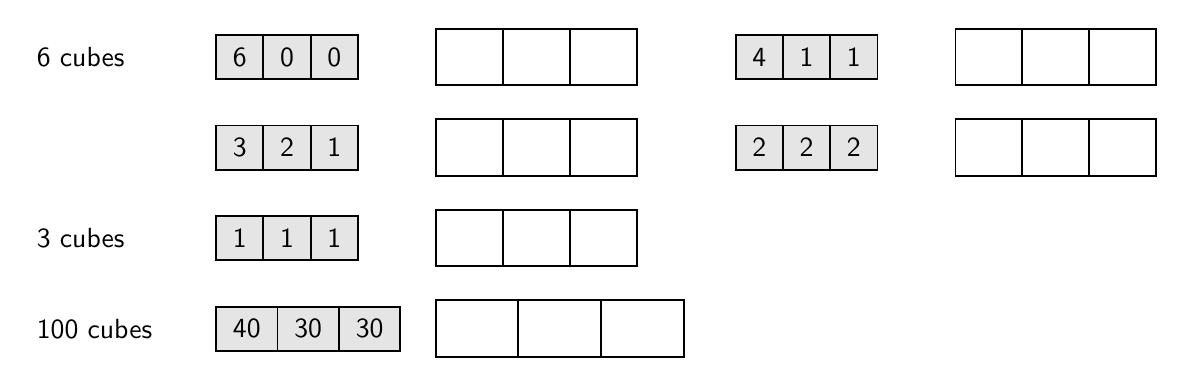
\begin{tikzpicture}[]
\node[anchor=west,font=\normalsize] at (0,0.360) {6 cubes};
\draw[line width=0.7pt,fill=black!10] (2.400,0.080) rectangle (3.000,0.640);
\node[font=\normalsize] at (2.700,0.360) {6};
\draw[line width=0.7pt,fill=black!10] (3.000,0.080) rectangle (3.600,0.640);
\node[font=\normalsize] at (3.300,0.360) {0};
\draw[line width=0.7pt,fill=black!10] (3.600,0.080) rectangle (4.200,0.640);
\node[font=\normalsize] at (3.900,0.360) {0};
\draw[line width=0.7pt] (5.190,0.000) rectangle (6.040,0.720);
\draw[line width=0.7pt] (6.040,0.000) rectangle (6.890,0.720);
\draw[line width=0.7pt] (6.890,0.000) rectangle (7.740,0.720);
\draw[line width=0.7pt,fill=black!10] (9.000,0.080) rectangle (9.600,0.640);
\node[font=\normalsize] at (9.300,0.360) {4};
\draw[line width=0.7pt,fill=black!10] (9.600,0.080) rectangle (10.200,0.640);
\node[font=\normalsize] at (9.900,0.360) {1};
\draw[line width=0.7pt,fill=black!10] (10.200,0.080) rectangle (10.800,0.640);
\node[font=\normalsize] at (10.500,0.360) {1};
\draw[line width=0.7pt] (11.790,0.000) rectangle (12.640,0.720);
\draw[line width=0.7pt] (12.640,0.000) rectangle (13.490,0.720);
\draw[line width=0.7pt] (13.490,0.000) rectangle (14.340,0.720);
\draw[line width=0.7pt,fill=black!10] (2.400,-1.070) rectangle (3.000,-0.510);
\node[font=\normalsize] at (2.700,-0.790) {3};
\draw[line width=0.7pt,fill=black!10] (3.000,-1.070) rectangle (3.600,-0.510);
\node[font=\normalsize] at (3.300,-0.790) {2};
\draw[line width=0.7pt,fill=black!10] (3.600,-1.070) rectangle (4.200,-0.510);
\node[font=\normalsize] at (3.900,-0.790) {1};
\draw[line width=0.7pt] (5.190,-1.150) rectangle (6.040,-0.430);
\draw[line width=0.7pt] (6.040,-1.150) rectangle (6.890,-0.430);
\draw[line width=0.7pt] (6.890,-1.150) rectangle (7.740,-0.430);
\draw[line width=0.7pt,fill=black!10] (9.000,-1.070) rectangle (9.600,-0.510);
\node[font=\normalsize] at (9.300,-0.790) {2};
\draw[line width=0.7pt,fill=black!10] (9.600,-1.070) rectangle (10.200,-0.510);
\node[font=\normalsize] at (9.900,-0.790) {2};
\draw[line width=0.7pt,fill=black!10] (10.200,-1.070) rectangle (10.800,-0.510);
\node[font=\normalsize] at (10.500,-0.790) {2};
\draw[line width=0.7pt] (11.790,-1.150) rectangle (12.640,-0.430);
\draw[line width=0.7pt] (12.640,-1.150) rectangle (13.490,-0.430);
\draw[line width=0.7pt] (13.490,-1.150) rectangle (14.340,-0.430);
\node[anchor=west,font=\normalsize] at (0,-1.940) {3 cubes};
\draw[line width=0.7pt,fill=black!10] (2.400,-2.220) rectangle (3.000,-1.660);
\node[font=\normalsize] at (2.700,-1.940) {1};
\draw[line width=0.7pt,fill=black!10] (3.000,-2.220) rectangle (3.600,-1.660);
\node[font=\normalsize] at (3.300,-1.940) {1};
\draw[line width=0.7pt,fill=black!10] (3.600,-2.220) rectangle (4.200,-1.660);
\node[font=\normalsize] at (3.900,-1.940) {1};
\draw[line width=0.7pt] (5.190,-2.300) rectangle (6.040,-1.580);
\draw[line width=0.7pt] (6.040,-2.300) rectangle (6.890,-1.580);
\draw[line width=0.7pt] (6.890,-2.300) rectangle (7.740,-1.580);
\node[anchor=west,font=\normalsize] at (0,-3.090) {100 cubes};
\draw[line width=0.7pt,fill=black!10] (2.400,-3.370) rectangle (3.180,-2.810);
\node[font=\normalsize] at (2.790,-3.090) {40};
\draw[line width=0.7pt,fill=black!10] (3.180,-3.370) rectangle (3.960,-2.810);
\node[font=\normalsize] at (3.570,-3.090) {30};
\draw[line width=0.7pt,fill=black!10] (3.960,-3.370) rectangle (4.740,-2.810);
\node[font=\normalsize] at (4.350,-3.090) {30};
\draw[line width=0.7pt] (5.190,-3.450) rectangle (6.240,-2.730);
\draw[line width=0.7pt] (6.240,-3.450) rectangle (7.290,-2.730);
\draw[line width=0.7pt] (7.290,-3.450) rectangle (8.340,-2.730);
\end{tikzpicture}
\par\vspace{10pt}\par\noindent
\begin{tikzpicture}\draw[black!30,line width=0.5pt] (0,-0.850) -- (\linewidth-1pt,-0.850);\draw[black!30,line width=0.5pt] (0,-1.700) -- (\linewidth-1pt,-1.700);\draw[black!30,line width=0.5pt] (0,-2.550) -- (\linewidth-1pt,-2.550);\draw[black!30,line width=0.5pt] (0,-3.400) -- (\linewidth-1pt,-3.400);\draw[black!30,line width=0.5pt] (0,-4.250) -- (\linewidth-1pt,-4.250);\end{tikzpicture}\par
\prob{7}Your partner has 6 cubes. What is the fewest cubes you need for a plan that your partner cannot beat? For a plan that beats every plan your partner could make?
\par\vspace{2pt}\par\noindent
\begin{tikzpicture}\draw[black!30,line width=0.5pt] (0,-0.850) -- (\linewidth-1pt,-0.850);\draw[black!30,line width=0.5pt] (0,-1.700) -- (\linewidth-1pt,-1.700);\draw[black!30,line width=0.5pt] (0,-2.550) -- (\linewidth-1pt,-2.550);\draw[black!30,line width=0.5pt] (0,-3.400) -- (\linewidth-1pt,-3.400);\draw[black!30,line width=0.5pt] (0,-4.250) -- (\linewidth-1pt,-4.250);\draw[black!30,line width=0.5pt] (0,-5.100) -- (\linewidth-1pt,-5.100);\draw[black!30,line width=0.5pt] (0,-5.950) -- (\linewidth-1pt,-5.950);\end{tikzpicture}\par
\newpage
\prob{8}Ben and Mia each choose a plan with 6 cubes by rolling a die and using the list below. You know their lists but not their rolls. For each of them, look for a plan with 6 cubes that beats more of their six plans than it loses to. If there is none, explain why.
\par\vspace{14pt}\noindent\hspace*{0.5cm}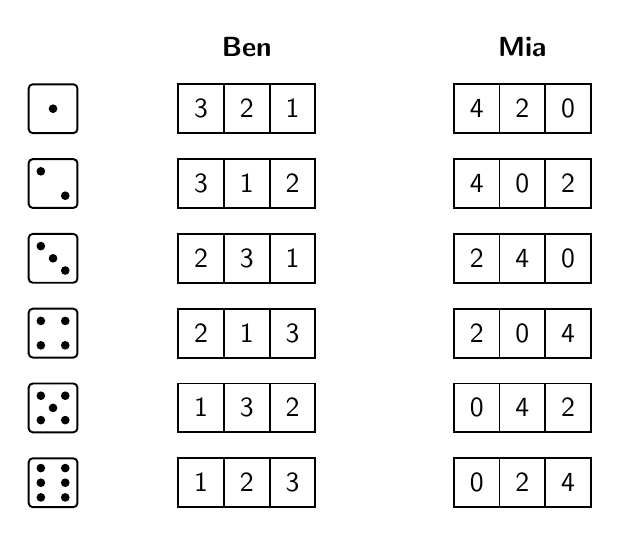
\begin{tikzpicture}[]
\node[font=\normalsize\bfseries] at (2.77,0.85) {Ben};
\node[font=\normalsize\bfseries] at (6.27,0.85) {Mia};
\draw[line width=0.7pt,rounded corners=1.5pt] (0.000,-0.250) rectangle (0.620,0.370);
\fill (0.310,0.060) circle (0.055);
\draw[line width=0.7pt] (1.900,-0.250) rectangle (2.480,0.370);
\node[font=\normalsize] at (2.190,0.060) {3};
\draw[line width=0.7pt] (2.480,-0.250) rectangle (3.060,0.370);
\node[font=\normalsize] at (2.770,0.060) {2};
\draw[line width=0.7pt] (3.060,-0.250) rectangle (3.640,0.370);
\node[font=\normalsize] at (3.350,0.060) {1};
\draw[line width=0.7pt] (5.400,-0.250) rectangle (5.980,0.370);
\node[font=\normalsize] at (5.690,0.060) {4};
\draw[line width=0.7pt] (5.980,-0.250) rectangle (6.560,0.370);
\node[font=\normalsize] at (6.270,0.060) {2};
\draw[line width=0.7pt] (6.560,-0.250) rectangle (7.140,0.370);
\node[font=\normalsize] at (6.850,0.060) {0};
\draw[line width=0.7pt,rounded corners=1.5pt] (0.000,-1.200) rectangle (0.620,-0.580);
\fill (0.155,-0.735) circle (0.055);
\fill (0.465,-1.045) circle (0.055);
\draw[line width=0.7pt] (1.900,-1.200) rectangle (2.480,-0.580);
\node[font=\normalsize] at (2.190,-0.890) {3};
\draw[line width=0.7pt] (2.480,-1.200) rectangle (3.060,-0.580);
\node[font=\normalsize] at (2.770,-0.890) {1};
\draw[line width=0.7pt] (3.060,-1.200) rectangle (3.640,-0.580);
\node[font=\normalsize] at (3.350,-0.890) {2};
\draw[line width=0.7pt] (5.400,-1.200) rectangle (5.980,-0.580);
\node[font=\normalsize] at (5.690,-0.890) {4};
\draw[line width=0.7pt] (5.980,-1.200) rectangle (6.560,-0.580);
\node[font=\normalsize] at (6.270,-0.890) {0};
\draw[line width=0.7pt] (6.560,-1.200) rectangle (7.140,-0.580);
\node[font=\normalsize] at (6.850,-0.890) {2};
\draw[line width=0.7pt,rounded corners=1.5pt] (0.000,-2.150) rectangle (0.620,-1.530);
\fill (0.155,-1.685) circle (0.055);
\fill (0.310,-1.840) circle (0.055);
\fill (0.465,-1.995) circle (0.055);
\draw[line width=0.7pt] (1.900,-2.150) rectangle (2.480,-1.530);
\node[font=\normalsize] at (2.190,-1.840) {2};
\draw[line width=0.7pt] (2.480,-2.150) rectangle (3.060,-1.530);
\node[font=\normalsize] at (2.770,-1.840) {3};
\draw[line width=0.7pt] (3.060,-2.150) rectangle (3.640,-1.530);
\node[font=\normalsize] at (3.350,-1.840) {1};
\draw[line width=0.7pt] (5.400,-2.150) rectangle (5.980,-1.530);
\node[font=\normalsize] at (5.690,-1.840) {2};
\draw[line width=0.7pt] (5.980,-2.150) rectangle (6.560,-1.530);
\node[font=\normalsize] at (6.270,-1.840) {4};
\draw[line width=0.7pt] (6.560,-2.150) rectangle (7.140,-1.530);
\node[font=\normalsize] at (6.850,-1.840) {0};
\draw[line width=0.7pt,rounded corners=1.5pt] (0.000,-3.100) rectangle (0.620,-2.480);
\fill (0.155,-2.945) circle (0.055);
\fill (0.155,-2.635) circle (0.055);
\fill (0.465,-2.945) circle (0.055);
\fill (0.465,-2.635) circle (0.055);
\draw[line width=0.7pt] (1.900,-3.100) rectangle (2.480,-2.480);
\node[font=\normalsize] at (2.190,-2.790) {2};
\draw[line width=0.7pt] (2.480,-3.100) rectangle (3.060,-2.480);
\node[font=\normalsize] at (2.770,-2.790) {1};
\draw[line width=0.7pt] (3.060,-3.100) rectangle (3.640,-2.480);
\node[font=\normalsize] at (3.350,-2.790) {3};
\draw[line width=0.7pt] (5.400,-3.100) rectangle (5.980,-2.480);
\node[font=\normalsize] at (5.690,-2.790) {2};
\draw[line width=0.7pt] (5.980,-3.100) rectangle (6.560,-2.480);
\node[font=\normalsize] at (6.270,-2.790) {0};
\draw[line width=0.7pt] (6.560,-3.100) rectangle (7.140,-2.480);
\node[font=\normalsize] at (6.850,-2.790) {4};
\draw[line width=0.7pt,rounded corners=1.5pt] (0.000,-4.050) rectangle (0.620,-3.430);
\fill (0.155,-3.895) circle (0.055);
\fill (0.155,-3.585) circle (0.055);
\fill (0.310,-3.740) circle (0.055);
\fill (0.465,-3.895) circle (0.055);
\fill (0.465,-3.585) circle (0.055);
\draw[line width=0.7pt] (1.900,-4.050) rectangle (2.480,-3.430);
\node[font=\normalsize] at (2.190,-3.740) {1};
\draw[line width=0.7pt] (2.480,-4.050) rectangle (3.060,-3.430);
\node[font=\normalsize] at (2.770,-3.740) {3};
\draw[line width=0.7pt] (3.060,-4.050) rectangle (3.640,-3.430);
\node[font=\normalsize] at (3.350,-3.740) {2};
\draw[line width=0.7pt] (5.400,-4.050) rectangle (5.980,-3.430);
\node[font=\normalsize] at (5.690,-3.740) {0};
\draw[line width=0.7pt] (5.980,-4.050) rectangle (6.560,-3.430);
\node[font=\normalsize] at (6.270,-3.740) {4};
\draw[line width=0.7pt] (6.560,-4.050) rectangle (7.140,-3.430);
\node[font=\normalsize] at (6.850,-3.740) {2};
\draw[line width=0.7pt,rounded corners=1.5pt] (0.000,-5.000) rectangle (0.620,-4.380);
\fill (0.155,-4.876) circle (0.055);
\fill (0.155,-4.690) circle (0.055);
\fill (0.155,-4.504) circle (0.055);
\fill (0.465,-4.876) circle (0.055);
\fill (0.465,-4.690) circle (0.055);
\fill (0.465,-4.504) circle (0.055);
\draw[line width=0.7pt] (1.900,-5.000) rectangle (2.480,-4.380);
\node[font=\normalsize] at (2.190,-4.690) {1};
\draw[line width=0.7pt] (2.480,-5.000) rectangle (3.060,-4.380);
\node[font=\normalsize] at (2.770,-4.690) {2};
\draw[line width=0.7pt] (3.060,-5.000) rectangle (3.640,-4.380);
\node[font=\normalsize] at (3.350,-4.690) {3};
\draw[line width=0.7pt] (5.400,-5.000) rectangle (5.980,-4.380);
\node[font=\normalsize] at (5.690,-4.690) {0};
\draw[line width=0.7pt] (5.980,-5.000) rectangle (6.560,-4.380);
\node[font=\normalsize] at (6.270,-4.690) {2};
\draw[line width=0.7pt] (6.560,-5.000) rectangle (7.140,-4.380);
\node[font=\normalsize] at (6.850,-4.690) {4};
\end{tikzpicture}
\par\vspace{6pt}\par\noindent
\begin{tikzpicture}\draw[black!30,line width=0.5pt] (0,-0.850) -- (\linewidth-1pt,-0.850);\draw[black!30,line width=0.5pt] (0,-1.700) -- (\linewidth-1pt,-1.700);\draw[black!30,line width=0.5pt] (0,-2.550) -- (\linewidth-1pt,-2.550);\draw[black!30,line width=0.5pt] (0,-3.400) -- (\linewidth-1pt,-3.400);\draw[black!30,line width=0.5pt] (0,-4.250) -- (\linewidth-1pt,-4.250);\draw[black!30,line width=0.5pt] (0,-5.100) -- (\linewidth-1pt,-5.100);\draw[black!30,line width=0.5pt] (0,-5.950) -- (\linewidth-1pt,-5.950);\draw[black!30,line width=0.5pt] (0,-6.800) -- (\linewidth-1pt,-6.800);\draw[black!30,line width=0.5pt] (0,-7.650) -- (\linewidth-1pt,-7.650);\draw[black!30,line width=0.5pt] (0,-8.500) -- (\linewidth-1pt,-8.500);\end{tikzpicture}\par

\end{document}
